%% Draft manuscript for the Planetary Science Journal
%% First draft 2026-07-03. Scaffolded sections are marked [To be completed: ...]
%% and with %%TODO comments. Numbers are drawn from the repository's committed
%% results (docs/capture_feasibility.md, docs/site_mc_findings.md,
%% results/sitemc_summary.json, results/bounce_off_phase_diagram.json).
\documentclass[twocolumn]{aastex631}

\usepackage{amsmath}
\graphicspath{{../figures/}}

\newcommand{\vinf}{v_{\infty}}
\newcommand{\RE}{R_{\oplus}}
\newcommand{\kms}{\ensuremath{{\rm \,km\,s^{-1}}}}

\shorttitle{Capture and Deorbit of Kilometer-Scale Iron Asteroids}
\shortauthors{Laughlin et al.}

\begin{document}

\title{The Capture and Deorbit of Kilometer-Scale Iron Asteroids}

\author[0000-0002-3253-2621]{Gregory Laughlin}
\affiliation{Department of Astronomy, Yale University, New Haven, CT 06511, USA}
%%TODO: author list and affiliations to be settled.

\begin{abstract}
A kilometer-scale metallic asteroid that encounters Earth with a small
hyperbolic excess velocity can be captured into a bound orbit by a single
grazing passage through the upper atmosphere. The ballistic coefficient of
such a body is enormous, $\beta = m/(C_{\rm D}A) \approx 5\times10^{6}\,{\rm
kg\,m^{-2}}$, so the braking accumulated during one periapsis passage is
slight; nevertheless, we show that the energy removed from a slow encounter
is sufficient for capture over a corridor of periapsis altitudes that is
tens of kilometers wide for $\vinf \lesssim 4$ \kms. A simple closed-form
expression, corrected for the curvature of a near-parabolic grazing arc,
reproduces the numerically determined capture boundary to a few percent.
The internal strength of the body enters decisively: at the periapsis
distances in question, a rubble pile is disrupted by tides while an intact
iron body survives with a wide margin, so that a single flyby geometry
bifurcates into a debris ring or a captured monolith according to the
constitution of the visitor. Captured orbits are pruned by the Moon; those
with first apogees below roughly a third of the lunar distance decay
through a rapid aerobraking cascade---typically days to weeks---and arrive
at the top of the atmosphere on trajectories inclined less than a few
degrees from the local horizontal. A Monte Carlo over $10^{6}$ arrival
geometries, integrated through capture, orbital decay, and terminal descent
onto a global elevation model with an atmosphere that follows the geoid,
yields the geography of the resulting impacts: half occur within
$15^{\circ}$ of the equator, ocean is struck almost in proportion to its
area, and the probability per unit area climbs monotonically with surface
elevation, reaching an enhancement of $2.75^{+0.53}_{-0.50}$ above 5 km.
Among named summits, Cayambe in Ecuador is the single most favored point
of impact on the planet, a distinction it owes to its latitude rather than
its height. We discuss the terminal grazing impact itself, for which
smoothed-particle simulations delineate ricochet, fragmentation, and escape
regimes, and we outline the application of these results to the
mid-Ordovician impact interval.
%%TODO: final sentence on event rate once the rate integral is done.
\end{abstract}

\keywords{Near-Earth objects (1092) --- Atmospheric entry (2320) ---
Impact phenomena (779) --- Orbital evolution (1178)}

\section{Introduction} \label{sec:intro}

The near-Earth population contains a small number of metallic asteroids of
kilometer scale. The largest confirmed example, (6178)~1986~DA, is a
radar-bright body roughly 2.7 km across whose surface is consistent with
$\sim$85\% metal \citep{sanchez2021}. Objects of this class are rare---they
constitute at most a few percent of the near-Earth census---but they are
qualitatively distinct from their stony relatives. A monolithic iron body
possesses material strength of order $10^{8}$--$10^{9}$ Pa, several orders
of magnitude beyond the gravitational binding stress of a kilometer-scale
rubble pile, and this strength permits it to survive encounters that would
disassemble an ordinary asteroid.

Our interest in such encounters has a specific geological motivation.
\citet{tomkins2024} have assembled evidence that Earth possessed a ring
during the Ordovician: a band of impact structures near the paleoequator, a
$\sim$40 Myr interval of enhanced extraterrestrial chondritic debris in
marine sediments \citep{schmitz2001}, and the coincidence of both with a
plausible tidal-disruption event. In their scenario, a large rubble-bodied
asteroid passed inside the Roche limit, was pulled apart, and the resulting
ring decayed onto the equatorial belt over tens of millions of years. The
scenario relies on the visitor being weak. It is natural to ask what
happens when the same encounter is experienced by a body that does not
come apart---a question that, so far as we have been able to determine,
has not been quantitatively examined at kilometer scale.

The dynamics of small bodies interacting with Earth's atmosphere has been
studied thoroughly in two regimes that bracket ours. At meter scale,
temporary capture is well understood: Earth maintains a steady-state
population of minimoons drawn from the slowest tail of the encounter
distribution \citep{granvik2012, fedorets2017}, and two such objects, 2006
RH$_{120}$ and 2020 CD$_{3}$, have been observed in geocentric orbits. At
50--200 m scale, calculations of iron bodies traversing the atmosphere on
hyperbolic trajectories find that they pass through, losing modest energy
\citep{khrennikov2020}. Meanwhile the impact-cratering literature treats
bodies that arrive steeply and terminally; the systematics of oblique
impacts have been mapped experimentally down to grazing angles where
projectiles ricochet \citep{gaultwedekind1978, schultzgault1990}, but the
coupling of that regime to a preceding orbital-decay history has not been
worked out. Between the minimoons and the craters lies an unexplored
channel: a kilometer-scale body of sufficient strength, arriving slowly,
braking by successive grazing passages, and ultimately striking the surface
at an angle of a degree or so. This paper is an attempt to characterize
that channel from encounter to ground.

The plan of the paper is as follows. In \S\ref{sec:capture} we treat the
capture problem analytically and numerically, and show that the corridor
for single-pass aerodynamic capture is narrow but by no means fine-tuned.
In \S\ref{sec:fate} we follow captured orbits through the three-body
environment, where the Moon eliminates the more weakly bound cases and the
survivors decay through a brief aerobraking cascade. In \S\ref{sec:geography}
we present a Monte Carlo over arrival geometries that yields the
statistical geography of the terminal impacts, and we isolate the dynamical
mechanisms responsible for its strong latitude dependence. In
\S\ref{sec:terminal} we consider the terminal grazing impact itself.
Section \ref{sec:discussion} estimates the frequency of such events,
applies the results to the Ordovician record, and collects the caveats.
Section \ref{sec:summary} summarizes.

\section{Aerodynamic Capture} \label{sec:capture}

\subsection{The character of the problem} \label{sec:character}

Consider an iron sphere of diameter 1 km and density $\rho_{\rm b} = 7800$
kg m$^{-3}$, so that $m = 4.1\times10^{12}$ kg and $A = 7.9\times10^{5}$
m$^{2}$. With a drag coefficient $C_{\rm D} = 1$, the ballistic
coefficient is
\begin{equation}
\beta \;=\; \frac{m}{C_{\rm D}A} \;=\; 5.2\times10^{6}\ {\rm kg\,m^{-2}},
\end{equation}
roughly four orders of magnitude beyond that of a re-entering spacecraft.
A body of this loading does not experience the atmosphere as an obstacle;
it experiences it as a faint, persistent drag. The essential question of
this section is whether a single periapsis passage deep enough to matter,
yet shallow enough to avoid the ground, can remove the modest specific
energy $\vinf^{2}/2$ that separates a slow hyperbolic encounter from a
bound orbit.

\subsection{The energy budget of a grazing passage} \label{sec:budget}

The mass of atmosphere traversed near periapsis controls the energy loss.
For a periapsis at altitude $h_{p}$, where the density is $\rho(h_{p})$ and
the local scale height is $H$, the familiar estimate of the traversed
column treats the trajectory as a parabola-over-a-sphere and integrates the
exponential atmosphere along the path, giving $\Sigma \simeq
\rho(h_{p})\sqrt{2\pi r_{p} H}$. This expression requires a correction
that, to our knowledge, is not usually made explicit. The radius of
curvature of a conic at periapsis is the semilatus rectum $p = r_{p}(1+e)$,
which for a near-parabolic graze is very nearly $2r_{p}$; the altitude
therefore rises along the path as $s^{2}/4r_{p}$ rather than
$s^{2}/2r_{p}$, and the body lingers in the dense layers $\sqrt{2}$ longer
than the naive estimate suggests:
\begin{equation}
\Sigma_{\rm eff} \;=\; \rho(h_{p})\,\sqrt{2\pi\,\tilde{r}\,H},
\qquad \tilde{r} = \frac{r_{p}\,p}{p - r_{p}} \simeq 2r_{p}.
\label{eq:column}
\end{equation}
The limiting cases behave sensibly: a circular orbit ($e \rightarrow 0$)
never leaves its density shell and $\tilde{r}$ diverges, while a fast
hyperbolic flyby ($e \gg 1$) approaches the straight-line column with
$\tilde{r} \rightarrow r_{p}$. Numerical integrations of single passages
through a piecewise-exponential model atmosphere \citep{vallado2013}
confirm the correction: over periapsis altitudes from 5 to 40 km, the
integrated energy loss exceeds the uncorrected estimate by factors of
1.38--1.42, in agreement with $\sqrt{2} = 1.414$ to within a few percent.

With the drag law $F = \tfrac{1}{2}\rho C_{\rm D} A v^{2}$, the speed lost
at periapsis is $\Delta v_{p} = v_{p}\Sigma_{\rm eff}/2\beta$, the orbital
energy removed is $v_{p}\,\Delta v_{p}$, and the condition for capture,
$v_{p}\Delta v_{p} > \vinf^{2}/2$, assumes the compact form
\begin{equation}
\vinf^{\rm max}(h_{p}) \;=\; v_{p}\,
\sqrt{\frac{\Sigma_{\rm eff}(h_{p})}{\beta}},
\label{eq:vinfmax}
\end{equation}
with $v_{p} \simeq \sqrt{2\mu_{\oplus}/r_{p}} \approx 11.2$ \kms\ for the
slow encounters of interest. Table~\ref{tab:corridor} compares this
expression with capture boundaries obtained by bisection on the full
numerical integrations. The agreement is at the level of a few percent
across an order of magnitude in $\vinf^{\rm max}$; the residual excess of
the numerical values at the lowest periapses reflects the modest additional
column encountered as drag lowers the actual periapsis below its vacuum
value during the pass.

\begin{deluxetable}{cccc}
\tablecaption{The capture boundary: closed form versus integration
\label{tab:corridor}}
\tablehead{
\colhead{$h_{p}$ (km)} & \colhead{$\Sigma_{\rm eff}$ (kg m$^{-2}$)} &
\colhead{Eq.~\ref{eq:vinfmax} (\kms)} & \colhead{numerical (\kms)}
}
\startdata
30 & $1.3\times10^{4}$ & 0.56 & 0.56 \\
20 & $5.9\times10^{4}$ & 1.19 & 1.18 \\
10 & $2.4\times10^{5}$ & 2.38 & 2.40 \\
5  & $4.7\times10^{5}$ & 3.35 & 3.42 \\
2  & $7.1\times10^{5}$ & 4.13 & 4.26 \\
\enddata
\end{deluxetable}

Two features of these numbers deserve emphasis. First, capture is possible
at all: a kilometer of solid iron can be brought into a bound orbit by air.
Second, the corridor is not razor-thin. A full sweep over the
$(\vinf, h_{p})$ plane finds capture extending to $\vinf = 4.2$ \kms, with
windows in periapsis altitude as wide as $\sim$40 km at low $\vinf$. A
Monte Carlo over the physically uncertain inputs---the drag coefficient of
a tumbling irregular body, the density of the lower atmosphere, its scale
height, and the sense of atmospheric co-rotation---places the 5th--95th
percentile range of the maximum capturable $\vinf$ at 3.2--5.6 \kms, with
the variance dominated by $C_{\rm D}$ (56\%) and the lower-atmosphere
density (40\%). It is worth noting that the periapsides that matter lie
between 2 and 45 km altitude, in the well-mixed lower and middle
atmosphere; the factor-of-several variability of the thermosphere, which
dominates the drag environment of artificial satellites, is irrelevant
here because a body of this ballistic coefficient does not feel the
thermosphere at all.
%%TODO: corridor map figure (v_inf vs h_p, colored by outcome, with the
%%ensemble envelope overplotted). Data exist in results/corridor_latest.json.

\subsection{Survival of the passage} \label{sec:survival}

Capture is useful only if the body arrives intact, and here the distinction
between a monolith and an aggregate is not a matter of degree. The peak
dynamic pressure on a capturing pass is $q = \tfrac{1}{2}\rho v_{p}^{2}
\approx 40$ MPa at $h_{p} = 5$ km. This is far below the crushing strength
of meteoritic iron ($\sim$0.1--0.5 GPa; octahedrite values from Canyon
Diablo material) and comparably far above the strength of any
gravitationally bound aggregate. Tides tell the same story with different
numbers. A grazing periapsis at $r_{p} = 1.001\,\RE$ lies well inside the
fluid Roche limit for $\rho_{\rm b} = 7800$ kg m$^{-3}$, which stands at
$2.17\,\RE$; the tidal stress across a kilometer body at periapsis,
$\sim$6 kPa, exceeds the $\sim$2 kPa self-gravitational central pressure of
a rubble pile of the same size, but falls eight orders of magnitude short
of threatening solid iron. A single flyby geometry therefore sorts
visitors by their constitution: the weak are disrupted into debris---the
opening act of the ring scenario of \citet{tomkins2024}---while the strong
proceed, captured and intact, into the aerobraking evolution that occupies
the remainder of this paper.

Ablation during the passage is negligible. Applying a Sutton-Graves
stagnation-point heating estimate over the $\sim$47 s of effective
atmospheric transit, and charging every joule of that heating to the
melting of iron with no radiative or convective relief, removes at most a
few centimeters of surface, a fractional mass loss below $10^{-3}$. The
thermal skin depth of iron over the passage time is likewise centimeters;
the interior never learns that the encounter happened.

\subsection{The supply of slow metallic encounters} \label{sec:supply}

Equation~\ref{eq:vinfmax} is of interest only if nature supplies metallic
bodies at $\vinf \lesssim 4$ \kms. Encounters this slow require orbits
that are nearly Earth-like: the Tisserand relation confines the
semilatus rectum of the heliocentric orbit to $\sqrt{a(1-e^{2})}\cos i
\simeq 1$, though it leaves the direction of the encounter velocity
usefully unconstrained (a point that matters for the geometry of capture,
and to which we return in \S\ref{sec:geography}). The observed minimoons
demonstrate that the slow tail is populated in the present-day solar
system, and the radar characterization of 1986~DA demonstrates that
kilometer-scale metal crosses near-Earth space. What the present epoch
does not obviously supply is the conjunction of the two. We take the view
that the calculation should establish the physical channel and its
branching fractions; the frequency question---how often per Gyr does a
kilometer-scale metallic body find itself in the capturable corner of
phase space---is deferred to \S\ref{sec:rate}, where it is treated by
folding the debiased near-Earth population models \citep{granvik2018,
nesvorny2023} against the corridor cross-section.
%%TODO [Section scaffold]: the rate integral. All machinery exists: the
%%corridor gives sigma(v_inf) = pi (b^2(h_max)-b^2(0)); the NEO model gives
%%the flux dN/dv_inf; the metallic fraction enters as a scalar.

\section{The Fate of Captured Orbits} \label{sec:fate}

\subsection{The Moon prunes the captures} \label{sec:moon}

A body captured by a single pass exits the atmosphere on a highly eccentric
ellipse whose apogee is set by how much energy the pass removed beyond the
capture threshold. Deep passes yield apogees of a few $\times10^{4}$ km;
marginal captures yield apogees approaching the lunar distance, and these
do not survive. Integrations in the full ephemeris environment (REBOUND
with the ASSIST force model: Sun, planets, Moon, Earth harmonics through
$J_{4}$; \citealt{rein2012, holman2023, park2021}) show that the Moon
imposes a sharp sorting on the first apogee. Orbits with first apogee
below $\sim$130,000 km---about a third of the lunar distance---aerobrake
gently to the grazing terminal state. Between $\sim$140,000 and 600,000
km, lunar perturbations drive the periapsis downward on orbital timescales,
converting the trajectory into a steep impact; a coasting test case with
apogee at 604,000 km had its periapsis carried from $+42$ km altitude to
$-2582$ km in a single 19.7-day orbit. Beyond $\sim2\times10^{6}$ km the
body is ejected. In the Monte Carlo of \S\ref{sec:geography}, 75\% of
captured-and-deorbited bodies took the gentle path, and the steep minority
carries a distinct signature (\S\ref{sec:latitude}).

\subsection{The aerobraking cascade} \label{sec:cascade}

The gentle captures then evolve with remarkable simplicity. Drag is
delivered almost entirely in the minute or two bracketing each periapsis
passage, and an impulse at periapsis lowers the opposite apsis; the orbit
therefore collapses along a sequence of ellipses of nearly constant
periapsis and shrinking apogee. In a representative case from the Monte
Carlo (an arrival with $\vinf = 1.5$ \kms\ captured at inclination
$48^{\circ}$; Figures~\ref{fig:traj} and \ref{fig:plane}), the body
executes 7 atmospheric passes over 2.06 days, with the first apogee at
68,400 km. The apsidal line barely moves while this happens: the apogee
directions of the successive passes span $0.7^{\circ}$, and the orbital
plane tilts by less than a degree, consistent with the modest $J_{2}$
apsidal and nodal rates at these element values. The cascade ends when the
apogee itself sinks into the atmosphere, at which point the trajectory
becomes a shallow, sub-orbital glide: in the case illustrated, the final
approach crosses the threshold of the atmosphere at 7.8 \kms\ descending at
$0.84^{\circ}$ below the local horizontal. Across the full Monte Carlo,
92\% of deorbited impactors arrive at flight-path angles shallower than
$5^{\circ}$; the terminal state of this channel is robustly a grazing
impact, a circumstance whose consequences occupy \S\ref{sec:terminal}.

An inclination is, for practical purposes, conserved through all of this.
Drag acts anti-parallel to the velocity and possesses no persistent
out-of-plane component beyond the small contribution of atmospheric
co-rotation; in the high-fidelity integrations the inclination changes by
less than $0.1^{\circ}$ over a complete cascade while $J_{2}$ regresses the
node through tens of degrees. A captured body therefore remembers the
inclination of its arrival geometry all the way to the ground, and
forgets everything else.

\begin{figure*}
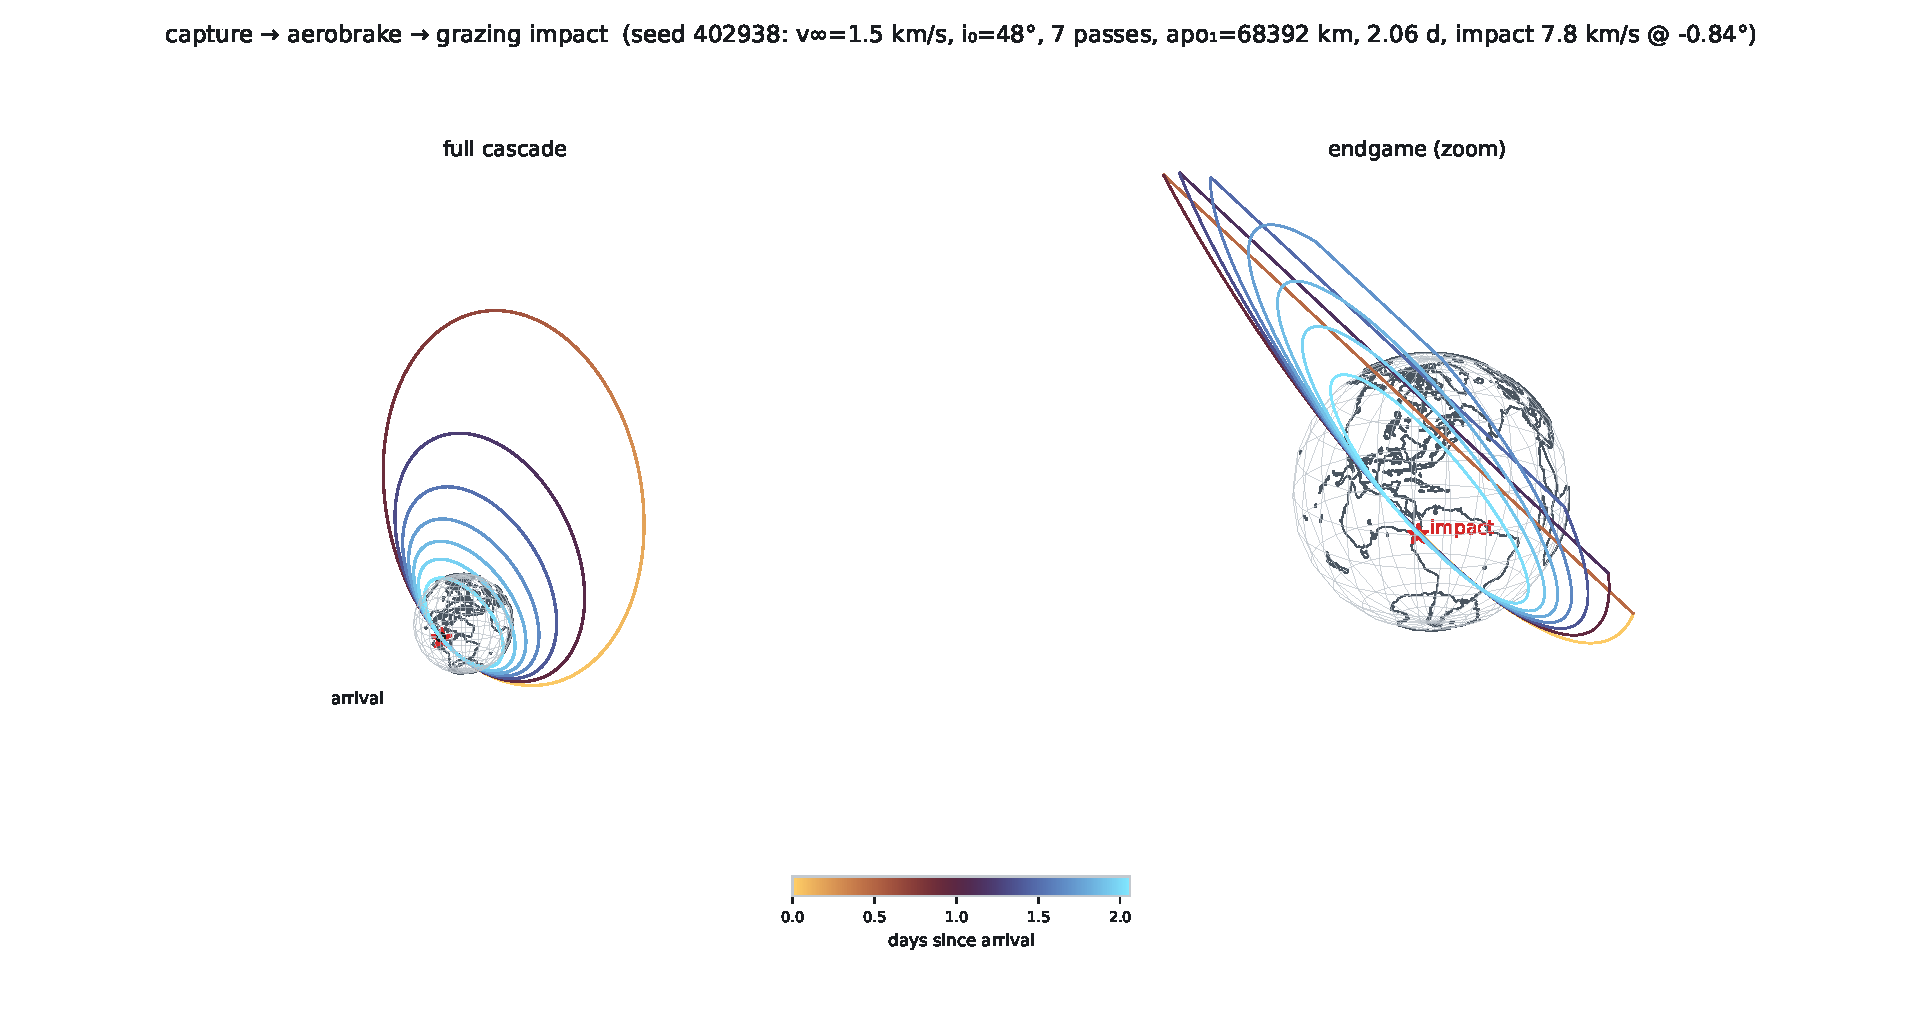
\includegraphics[width=\textwidth]{sitemc_traj.pdf}
\caption{A representative capture and deorbit, rendered in perspective
(the occultation of the trajectory by the planet is computed along the
line of sight). Left: the full cascade---the arrival hyperbola and seven
successively smaller ellipses, colored by time. Right: the final passes
and the terminal grazing approach. The star marks the impact point, 78 km
from the summit of Cayambe in the Ecuadorian Andes.}
\label{fig:traj}
\end{figure*}

\begin{figure*}
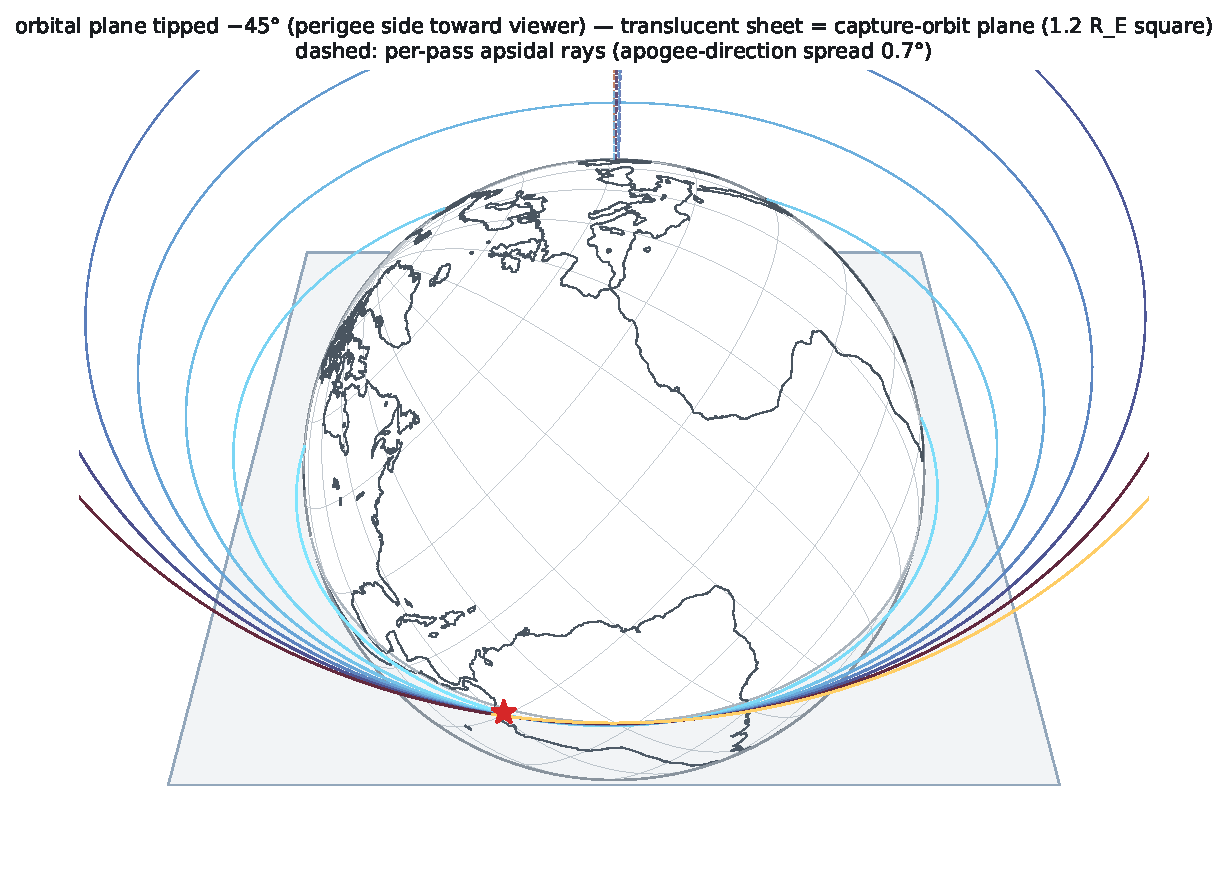
\includegraphics[width=\textwidth]{sitemc_traj_plane.pdf}
\caption{The same trajectory viewed $45^{\circ}$ from the normal to the
capture plane. The translucent sheet spans 1.1 times the semi-axes of the
largest bound orbit and lies in the plane of capture; dashed lines mark
the apsidal direction (whose total drift over the cascade is
$0.7^{\circ}$) and the perpendicular in-plane direction. The broad arrows
indicate the direction of orbital motion (on the incoming hyperbola) and
of Earth's rotation, which carries the surface through 2.1 revolutions
beneath the orbit during the 2.06-day cascade.}
\label{fig:plane}
\end{figure*}

\section{The Geography of Impact} \label{sec:geography}

\subsection{A Monte Carlo over arrivals} \label{sec:mc}

Where does such a body come down? The question is well posed because the
dynamics that follow capture are deterministic; what is statistical is the
arrival geometry. We therefore constructed a Monte Carlo in which each
trial is a single trajectory flown without interruption from the incoming
asymptote to the ground. The integrator is a geocentric formulation
carrying Earth's monopole and $J_{2}$, lunar and solar point-mass
perturbations from compact analytic ephemerides \citep{montenbruckgill},
and drag against a co-rotating atmosphere. Two features of the
implementation matter for the results and are worth stating plainly.

First, the atmosphere is oblate. Atmospheric density is evaluated at the
altitude above the reference ellipsoid, not above a sphere. The
equator-to-pole difference in geocentric radius, 21.4 km, amounts to three
scale heights of the lower atmosphere---a factor of $\sim$20 in density at
fixed distance from Earth's center---and for an inclined orbit decaying at
grazing altitudes this asymmetry, together with the $J_{2}$ figure of the
gravity field, controls where along the orbit the energy is spent.

Second, the terminal impact is registered against real topography. We
carry a global relief model \citep{amante2009} at one arc-minute
resolution, with the sharpest summits restored from a curated table (a
one arc-minute grid shaves several hundred meters from peaks of Alpine
sharpness), and terminate each trajectory when its geocentric radius
drops to that of the local terrain.

Each trial draws an arrival direction isotropically, an excess velocity
uniformly between 0.2 and 5 \kms, an impact parameter spanning the
capture corridor, a drag coefficient and atmospheric perturbation from
the uncertainty distributions of \S\ref{sec:budget}, and an epoch (hence
lunar phase and sidereal orientation) at random. All draws are recorded,
so that any astronomically motivated arrival distribution can be imposed
afterward by reweighting rather than by re-integration; we return to this
in \S\ref{sec:prior}. One million arrivals were flown. Of these, 89.8\%
escaped after their pass, 4.3\% struck the ground directly on the first
encounter, and 3.3\% (32,734 trajectories) were captured and subsequently
deorbited; the remaining 2.6\% were still in bound orbits when the
integrations were truncated at 200 days.

\subsection{The latitude rule} \label{sec:latitude}

The deorbited impacts are strongly concentrated toward the equator. The
quartiles of $|{\rm latitude}|$ fall at $7.5^{\circ}$, $15.2^{\circ}$, and
$25.1^{\circ}$, with 90\% of impacts within $36^{\circ}$; for comparison,
impacts spread uniformly over the sphere would place the median at
$30^{\circ}$. The concentration is not primarily a matter of which
terrain is tallest. Controlled experiments with the latitude dependence
of the atmosphere switched off (a spherically stratified atmosphere
referenced to the equatorial radius) retain most of the effect: the
equatorward drift is largely the work of $J_{2}$ on the orbit itself.
A near-circular orbit in an oblate field rides only 7--9 km of the 21.4 km
equator-to-pole figure of the geoid, so as the orbit shrinks, its low
points---where the remaining energy is spent---migrate toward the
equatorial bulge. The oblateness of the atmosphere then sharpens the
same tendency by roughly a third. The steep, Moon-pumped minority of
impacts shows a visibly broader latitude distribution, reaching into the
middle latitudes that the grazing channel rarely touches
(Figure~\ref{fig:map}).

It is worth recording what does \emph{not} happen. In an earlier and more
intuitive version of the site-selection argument, we imagined the decaying
body slowly combing the band of latitudes accessible to its inclination,
with the highest terrain in the band eventually intercepting the slowly
descending periapsis. The integrations decline to cooperate: the
discrimination window between the highest summits and sea level is
crossed in a median of two periapsis passes, so no such patient search
occurs. The latitude rule arises from the orbit dynamics; the terrain
selects only within the final descent.

\begin{figure*}
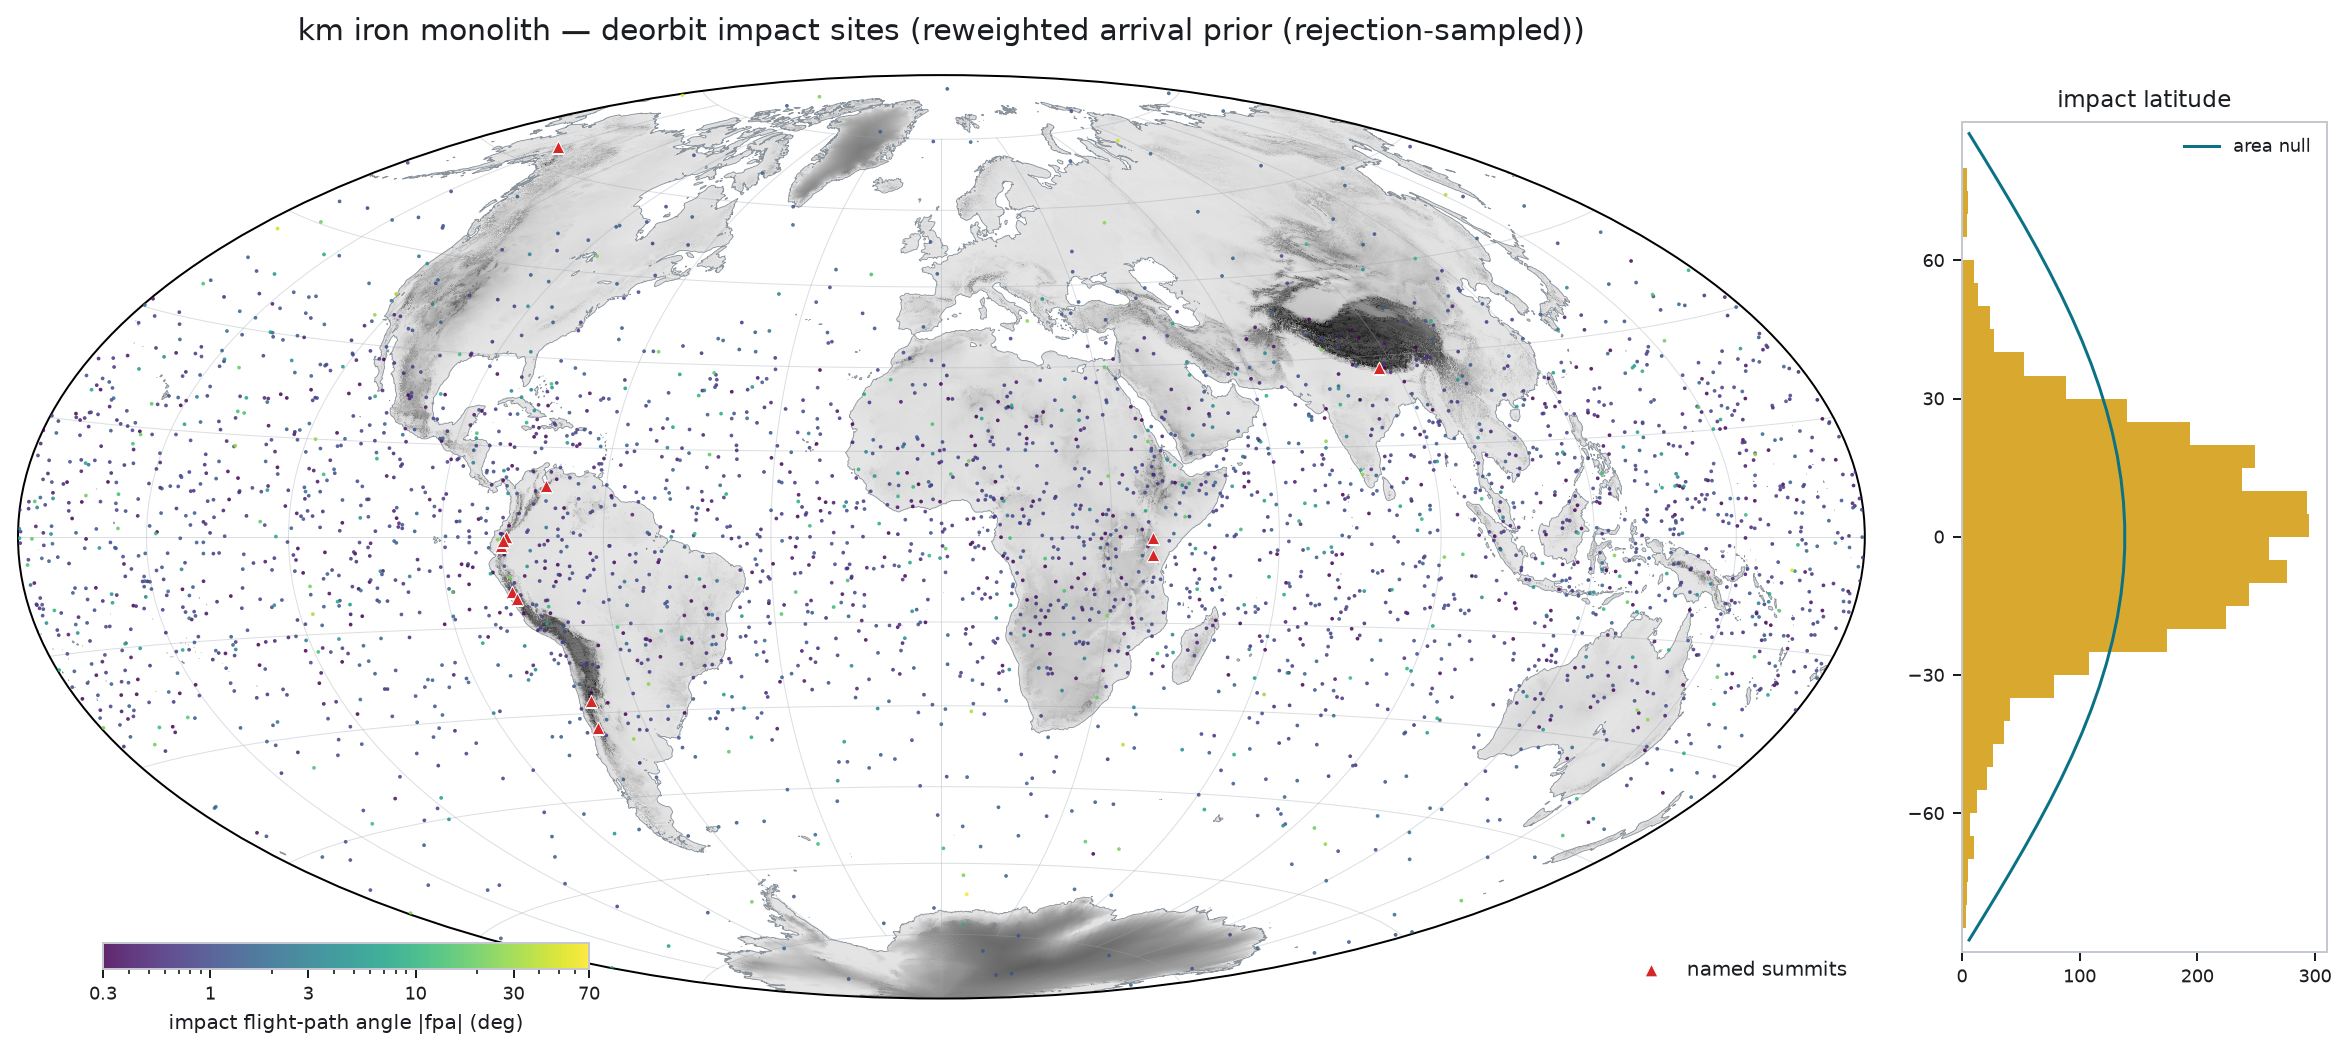
\includegraphics[width=\textwidth]{sitemc_flashlight_rw.pdf}
\caption{Impact locations for the captured-and-deorbited channel, drawn
from the Monte Carlo reweighted to the empirical arrival distribution of
Appendix~\ref{app:prior} (rejection-sampled so that the plotted density
of points is faithful). Points are colored by the magnitude of the
flight-path angle at impact, on a logarithmic scale from $0.3^{\circ}$
(grazing) to $70^{\circ}$; the steep tail is the Moon-pumped population
of \S\ref{sec:moon}. The right panel shows the latitude distribution
against the cosine law expected for uniform coverage.}
\label{fig:map}
\end{figure*}

\subsection{Elevation selection} \label{sec:elevation}

Within a latitude band, does high ground attract impacts beyond its share
of the map? The natural statistic is the ratio $\eta$ of the fraction of
impacts landing in a given elevation class to the area fraction of that
class, computed with the latitude distribution held fixed (so that the
latitude rule of the previous subsection cannot masquerade as an
elevation preference). Table~\ref{tab:eta} gives the result. Ocean is
struck almost, but not quite, in proportion to its area; the deficit,
4\%, is significant at the sample size and reappears as a mild excess on
land. The enhancement then climbs steadily with elevation, reaching
$2.15 \pm 0.18$ for terrain between 3 and 5 km and $2.75^{+0.53}_{-0.50}$
above 5 km.

\begin{deluxetable}{lcccc}
\tablecaption{Elevation selection at fixed latitude \label{tab:eta}}
\tablehead{
\colhead{class} & \colhead{$P_{\rm impact}$} & \colhead{$P_{\rm area}$} &
\colhead{$\eta$} & \colhead{95\% interval}
}
\startdata
ocean      & 0.714  & 0.742  & 0.96 & 0.96--0.97 \\
0--1 km    & 0.205  & 0.207  & 0.99 & 0.97--1.01 \\
1--3 km    & 0.063  & 0.043  & 1.45 & 1.38--1.52 \\
3--5 km    & 0.015  & 0.0070 & 2.15 & 1.97--2.33 \\
$>$5 km    & 0.0032 & 0.0012 & 2.75 & 2.25--3.28 \\
\enddata
\tablecomments{Computed from 32,734 deorbited impacts; the area
distribution is reweighted to the impact latitude distribution in
$2^{\circ}$ bands. Intervals are bootstrap.}
\end{deluxetable}

The mechanism is easily seen in individual trajectories. The illustrative
case of \S\ref{sec:cascade} spends its final 300 km of ground track
descending from 7.5 km altitude over the open Pacific, crosses the
Ecuadorian coastline at 4.6 km, and is met by the western rampart of the
Andes: over the last 30 km the terrain beneath it rises 2000 m while the
trajectory, descending at $0.84^{\circ}$, gives up only 400 m. The
mountains do the intercepting. A glide slope of a degree corresponds to
descending 6 km of altitude over $\sim$340 km of track, so any range that
rises kilometers over tens of kilometers presents a cross-section several
times its map area---which is essentially the factor that
Table~\ref{tab:eta} reports. By the same token, an isolated summit cone
gains little beyond its elevation class: the enhancement saturates at the
scale of the range that carries the summit, and we find no additional
spike attributable to the peaks themselves.

The named summits nevertheless order themselves instructively. Counting
impacts landing within 150 km of each of the twenty highest-geocentric-radius
summits, Cayambe in Ecuador leads the world with 26 of the 32,734
impacts---ahead of Everest (17, collected mostly by the broad shoulder of
the Tibetan Plateau), Huascar\'an (14), Kilimanjaro (13), and Chimborazo
(7). Cayambe's distinction is its address: it stands at $0.03^{\circ}$N,
at the very peak of the impact latitude distribution, on a cordillera
that faces the planet's longest stretch of open ocean. Height alone does
not decide these rankings; Chimborazo, though taller and possessed of the
greatest geocentric radius of any summit on Earth, sits $1.5^{\circ}$
south and collects a quarter of Cayambe's share.

\subsection{Robustness to the arrival distribution} \label{sec:prior}

The results above were computed under an isotropic arrival prior, and one
may reasonably object that real slow encounters arrive with a structured
distribution of directions. The objection can be met quantitatively.
Because every trial records its arrival draw, the catalog can be
reweighted to any prior; Appendix~\ref{app:prior} describes an empirical
construction in which heliocentric orbits are sampled from the Earth-like
corner of the near-Earth distribution and their encounter-velocity vectors
are accumulated at Earth's orbit, recovering the Tisserand kinematics
without recourse to closed-form encounter theory. Reweighting the catalog
to this distribution changes remarkably little: the latitude quartiles
move by a few tenths of a degree, the $\eta$ ladder is unchanged within
its intervals, and the effective sample size remains 89\% of the raw
count. The reason is that the Tisserand constraint, while pinning the
magnitude of the encounter velocity, leaves its direction broadly
distributed---slow arrivals are not confined near the ecliptic, and
capture inclinations up to and beyond $60^{\circ}$ remain well populated
under the realistic prior. The geography of Table~\ref{tab:eta} and
Figure~\ref{fig:map} is a property of the dynamics, not of the assumed
population; the population enters chiefly through the overall event rate.

\section{The Terminal Grazing Impact} \label{sec:terminal}

The deorbit channel delivers its impactor to the top of the atmosphere at
7--8 \kms\ on a trajectory a degree or so below horizontal. What follows
is neither a crater in the familiar sense nor a meteoric airburst: the
normal component of the impact velocity is of order 100 m s$^{-1}$, while
the tangential component remains hypersonic. The appropriate framework
is that of oblique-impact experiments extended to extreme incidence
\citep{gaultwedekind1978, schultzgault1990}, and the governing parameters
are the impact angle $\theta$ (measured from the horizontal) and the
speed in units of the escape velocity.

We have mapped this plane with a series of 69 three-dimensional
smoothed-particle hydrodynamics simulations of a kilometer-scale iron
sphere striking a basalt half-space, at resolutions of $\sim$6 million
particles, classifying each outcome as cratering, intact ricochet,
dispersed (shock-melted) ricochet, or escape of projectile material
\citep[methods follow][]{monaghan1992}. Three boundaries organize the
plane. Cratering---burial and arrest of the projectile---onsets only for
$\theta \gtrsim 36^{\circ}$ at $v/v_{\rm esc} = 1$, consistent with the
laboratory ricochet threshold near $30^{\circ}$
\citep{gaultwedekind1978}. Below that angle the projectile skips. Whether
it survives the skip intact is a question of shock heating: the
intact-to-dispersed boundary falls from $v/v_{\rm esc} \approx 0.96$ at
$\theta = 2^{\circ}$--$5^{\circ}$ to $\approx 0.60$ by $12^{\circ}$, as
steeper contact drives the leading face of the projectile past the
shock-melting threshold of iron. Escape of material to space requires
$v/v_{\rm esc} \gtrsim 1.1$ even at $\theta = 2^{\circ}$, and the escaping
material is in every such case molten or fragmented---an intact body
cannot be launched to escape by a grazing impact, because the contact
pressures required exceed the melting threshold, in accord with the
conclusions of \citet{pierazzomelosh2000}.

Two reality checks anchor the classification. Placing the Barringer
impactor (an iron mass arriving at $45^{\circ}$ and $v/v_{\rm esc} = 1.14$)
on the diagram yields cratering with complete projectile destruction, as
observed; placing Campo del Cielo ($\sim$$9^{\circ}$, $v/v_{\rm esc} =
0.31$) yields a coherent low-loss ricochet, consistent with the shallow
elongated penetration funnels and the survival of large masses at that
site. The deorbit channel's terminal state ($\theta \approx 1^{\circ},
v/v_{\rm esc} \approx 0.7$) falls deep in the intact-ricochet regime: the
first surface contact of a captured iron mountain is a touch-and-go.

\begin{figure}
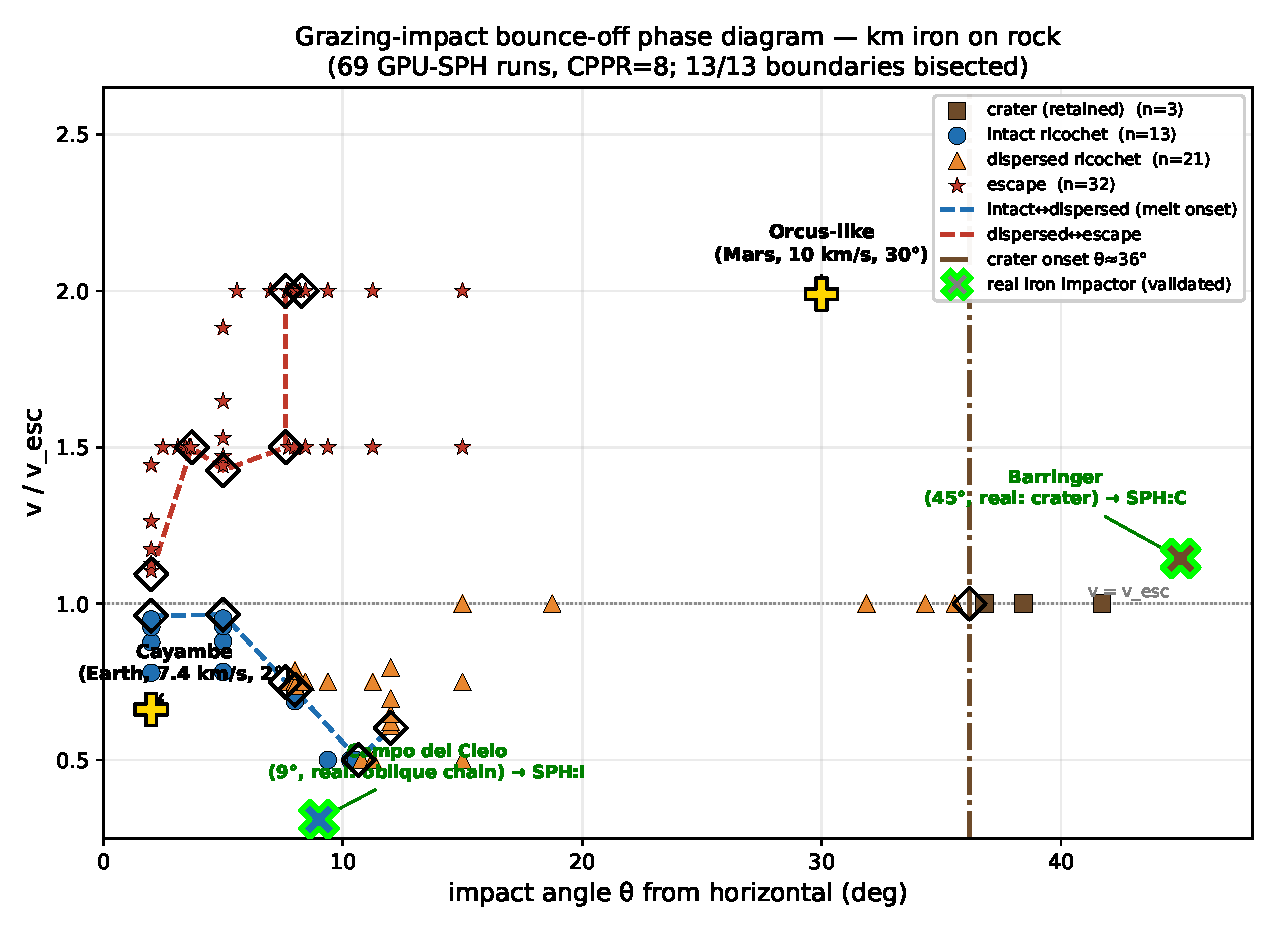
\includegraphics[width=\columnwidth]{bounce_off_phase_diagram.pdf}
\caption{The outcome plane for a kilometer-scale iron impactor on rock,
from 69 SPH simulations: cratering (C), intact ricochet (I), dispersed
ricochet (D), and escape of (molten) projectile material (E). The two
labeled points are the validation cases discussed in the text; the
terminal state of the deorbit channel lands in regime I.}
\label{fig:phase}
\end{figure}

\textit{[To be completed: the post-ricochet arc and second impact. Our
exploratory simulations of the Cayambe-class first contact indicate
decapitation of the summit topography, retention of $\sim$85\% of the
projectile's speed, partial melting, and a suborbital arc carrying the
debris $\sim$3000 km downrange; the surviving material re-enters as a
dispersed train rather than a coherent body, depositing a spherule-rich
strewn field of continental dimensions. These simulations require a
resolution study and a treatment of aerodynamic dispersal during the arc
before their quantitative features can be asserted. This subsection will
present them, together with the energy budget delivered to the atmosphere
and surface along the multi-thousand-kilometer terminal track.]}
%%TODO: second-impact subsection; figures from the SPH campaign exist in
%%the repository (fragmentation/ribbon renders) pending the convergence runs.

\section{Discussion} \label{sec:discussion}

\subsection{How often?} \label{sec:rate}

\textit{[To be completed: the event-rate integral. The corridor
cross-section of \S\ref{sec:capture}, $\sigma(\vinf) = \pi
[b^{2}(h_{p}^{\rm max}) - b^{2}(0)]$ including gravitational focusing, is
to be folded against the debiased flux of near-Earth objects in the slow
tail \citep{granvik2018, nesvorny2023} and the metallic fraction of the
kilometer-scale population. An order-of-magnitude preview: the corridor
occupies a fraction $\sim10^{-2}$ of encounters slower than 4 \kms, the
slow tail itself is a small fraction of all Earth encounters, and
kilometer-scale metallic bodies number a few percent of a population that
delivers such encounters at a known rate. The interval between events of
the kind treated here plausibly exceeds a Gyr, which is long, but not long
compared to the Phanerozoic record against which the predicted signatures
would be sought.]}

\subsection{The Ordovician, rings, and monoliths} \label{sec:ordovician}

\textit{[To be completed once \S\ref{sec:rate} is in hand. The elements to
be assembled: (i) the ring scenario of \citet{tomkins2024} and the
L-chondrite delivery interval \citep{schmitz2001} establish that the
mid-Ordovician featured at least one slow, disruptive encounter; (ii) the
strength bifurcation of \S\ref{sec:survival} implies that the same
encounter environment, sampled by a strong body, produces the deorbit
channel computed here; (iii) the predicted signatures differ sharply---an
equatorial band of small decaying-ring impacts versus a single grazing
mega-track with a downrange spherule field---and the stratigraphic record
is capable in principle of distinguishing them. The paleogeographic
placement (which cordilleras stood near the Ordovician equator) belongs
here as well. Paleo-Earth parameters modify the quantitative results only
mildly: a Moon a few percent closer tightens the apogee filter of
\S\ref{sec:moon} proportionally, and a faster spin enters through the
co-rotation term, which carries three percent of the corridor variance.]}

\subsection{Caveats} \label{sec:caveats}

Several limitations of the present treatment should be kept in view.
The drag coefficient of a tumbling, irregular metallic body in hypersonic
rarefied-to-continuum transition is uncertain at the factor-of-two level,
and it dominates the error budget of the corridor width. The 200-day
truncation of the Monte Carlo leaves 2.6\% of captures unresolved; most of
these are Moon-perturbed orbits whose eventual disposition (impact or
escape) would modestly adjust the branching fractions but not the
geography. The atmosphere model is a static climatology; we have verified
that its latitude structure matters (\S\ref{sec:latitude}) and represented
that structure by the figure of the geoid, but seasonal and diurnal
variability of the lower atmosphere is unmodeled, and enters the same
error budget as the density uncertainty already carried. The elevation
statistics inherit the smoothing of a one arc-minute terrain grid,
partially corrected at the sharpest summits. Finally, the SPH outcome
boundaries of \S\ref{sec:terminal} are drawn at a single resolution;
their convergence study is in progress.
%%TODO: update caveat list as items are retired.

\section{Summary} \label{sec:summary}

A kilometer-scale iron asteroid arriving at Earth with a hyperbolic excess
below about 4 \kms\ can be captured by a single grazing pass through the
atmosphere, survives that pass by an enormous margin of strength, and---
provided the Moon does not intervene---spirals to the surface within days
along a cascade of ellipses whose apsidal line scarcely moves. Its impact,
when it comes, is a grazing one, delivered at 7--8 \kms\ within a few
degrees of horizontal, preferentially within $15^{\circ}$ of the equator,
on ocean nearly in proportion to ocean's extent, and on high terrain in
marked disproportion: mountain ranges present several times their map
area to a trajectory descending at a degree. Among the world's named
summits, the most probable single point of impact is Cayambe, on the
equator in Ecuador; the distinction belongs to its latitude and to the
Pacific approach that its cordillera commands, not to its altitude. The
first contact of such an impactor is a ricochet, and the eventual fate of
the body---dispersal along a downrange track of continental length---is
the subject of work in progress. The channel described here is
undoubtedly rare; but the record of the Phanerozoic is long, its
equatorial mountain belts are persistent features, and a signature
without a recognized process is an invitation to look again.

\begin{acknowledgments}
%%TODO: acknowledgments, funding, computing.
The numerical work reported here was performed with an open reproduction
package; all integrators, the Monte Carlo driver, and the analysis
pipeline, together with their verification suites, are available at
\url{https://github.com/oklo/deorbit}.
\end{acknowledgments}

\appendix

\section{An empirical arrival distribution} \label{app:prior}

The reweighting of \S\ref{sec:prior} requires the joint distribution of
encounter velocity vectors for slow Earth encounters. Rather than adopt
closed-form \"Opik--Wetherill encounter statistics, whose singular factors
invite implementation error, we construct the distribution numerically.
Heliocentric orbits are drawn from a density over $(a, e, i)$ confined to
the Earth-like region ($0.8 \le a/{\rm AU} \le 1.3$, $e \le 0.35$, $i \le
15^{\circ}$); orbital phases are drawn uniformly; and each sampled
configuration lying within a thin torus about Earth's orbit contributes
its velocity relative to the local circular motion to the accumulated
distribution. Because the samples are drawn uniformly in time, the
accumulation automatically weights each orbit by its residence probability
near 1 AU, and the classic kinematic factors emerge of their own accord;
we verify that every accumulated encounter speed satisfies the Tisserand
relation for its parent orbit to better than one percent. The resulting
velocity-space density, smoothed with a Gaussian kernel, supplies the
per-trial weight
$w \propto f(\mathbf{U})\,U^{3}\,db^{2}/dh_{p}$, where the geometric
factors convert the Monte Carlo's sampling measure (isotropic in
direction, uniform in speed and in periapsis altitude) to a physical flux
through the corridor annulus. Two bracketing choices of the population
density over the Earth-like region---uniform, and a tilt shaped to the
debiased models---yield indistinguishable geographic statistics, which is
the basis for the statement in \S\ref{sec:prior} that the map is
prior-robust.
%%TODO: replace the shaped tilt with a direct ingestion of the NEOMOD
%%grid when the rate integral of sec 6.1 is assembled.

\bibliography{references}
\bibliographystyle{aasjournal}

\end{document}
